 \documentclass[a4paper]{article}

%% Language and font encodings
\usepackage[english]{babel}
\usepackage[utf8x]{inputenc}
\usepackage[T1]{fontenc}
\usepackage{helvet}
%\usepackage[numbers]{natbib}
\usepackage[round]{natbib}
%% For citations with atuhor et al year, usehttps://www.overleaf.com/16365895fcrtzrvgdsvp
%% \usepackage[round]{natbib}
%% \bibliographystyle{abbrv} (optional)
%% \citealt{adams1995hitchhiker}
\usepackage{upgreek} %%% This enables non-italic greek letters.
%% The lowercase letters are named \upalpha, \upbeta, ... and so, and upercase are named \Upalpha, \Upbeta, ...
%% line thickness
\usepackage{soul} %% Highlight package
\usepackage{lineno} %% Add line numbers to the document

%% Sets page size and margins
\usepackage[a4paper,top=3cm,bottom=2cm,left=3cm,right=3cm,marginparwidth=1.75cm]{geometry}
\setlength{\arrayrulewidth}{0.5mm}
\setlength{\tabcolsep}{4pt}

\renewcommand{\arraystretch}{1.3}
\newcommand{\beq}{\begin{equation}}
\newcommand{\eeq}{\end{equation}}

%% Useful packages

\usepackage{lipsum}
\usepackage{amsmath}
\usepackage{graphicx}
\usepackage[colorinlistoftodos]{todonotes}
\usepackage[colorlinks=true, allcolors=blue]{hyperref}
\usepackage{array}
\usepackage{float}
\usepackage{appendix} 
\usepackage{multirow}
\usepackage[symbol]{footmisc}
\usepackage{setspace}
\usepackage{authblk} %%% Support for footnote style author/affiliation.
\usepackage{ctable}
\renewcommand{\thefootnote}{\fnsymbol{footnote}}
\renewcommand\Affilfont{\itshape\small}
\usepackage{comment}
\usepackage{subfig}  
\usepackage{subcaption}
\usepackage{indentfirst}
\usepackage{siunitx}
\usepackage{amssymb,stmaryrd}
\usepackage{bbold}
\usepackage{enumerate}
\usepackage{enumitem}
\bibliographystyle{dinat}
\usepackage{amsthm}
\usepackage{bm}
%%% Packages for theorems and definitions, etc

\newtheorem{corollary}{Corollary}[section]
\newtheorem{lemma}{Lemma}[section]
\theoremstyle{definition}
\newtheorem{definition}{Definition}[section]
\newtheorem{theorem}{Theorem}

\title{Comp Set 1}
\author[1]{Antonio Cobarrubia}
\affil[1]{Department of Physics, San Diego State University, San Diego, CA 92182}

\date{}

\begin{document}

\maketitle

\doublespacing


\section{Problem 1}
For this problem we used random walk of a confined two-dimensional confined lattice to simulate ergodic process. The lattice was assumed to be a square with a linear size (total length of an axis) to be 10, where there was equal possibility for all configurations. Let's consider a configuration M(i,j) where at (i',j') the M(i,j) = M(i,j) + 1.

For a 1000-steps, I found the minimum value of M(i,j) to be 0 and the maximum to be 40 (min(M(i,j)) = 0 and max(M(i,j)) = 40). I found the average of the configurations to be 10 with a standard deviation of 7.6 ($<M(i,j)>$ = $10 \pm 7.6$).

For 8000-steps, I found the minimum amount of configuration to be 48 while the maximum value to be 124 (min(M(i,j)) = 48 and max(M(i,j)) = 124). The average amount of configurations for these amount of steps was 80 with a standard deviation of 15.4 ($<M(i,j)>$ = $80 \pm 15.4$).

To truly determine this algorithm is ergodic process, we need to see if a plot of standard deviation over the average of M versus heads to zero as the number of steps increases. Or in other words we need to plot standard deviation per average of M versus number of steps. An ergodic process is when the average at a certain sample time is the same as the average of over the whole process. A non ergodic process will have no predicted behavior and therefore have a mean always to zero. This means for our process the system will be ergodic if the ratio of standard deviation per average converges to zero since this plot will tell us if our confined lattice has predictive behavior.

\begin{figure}[H]
\centering
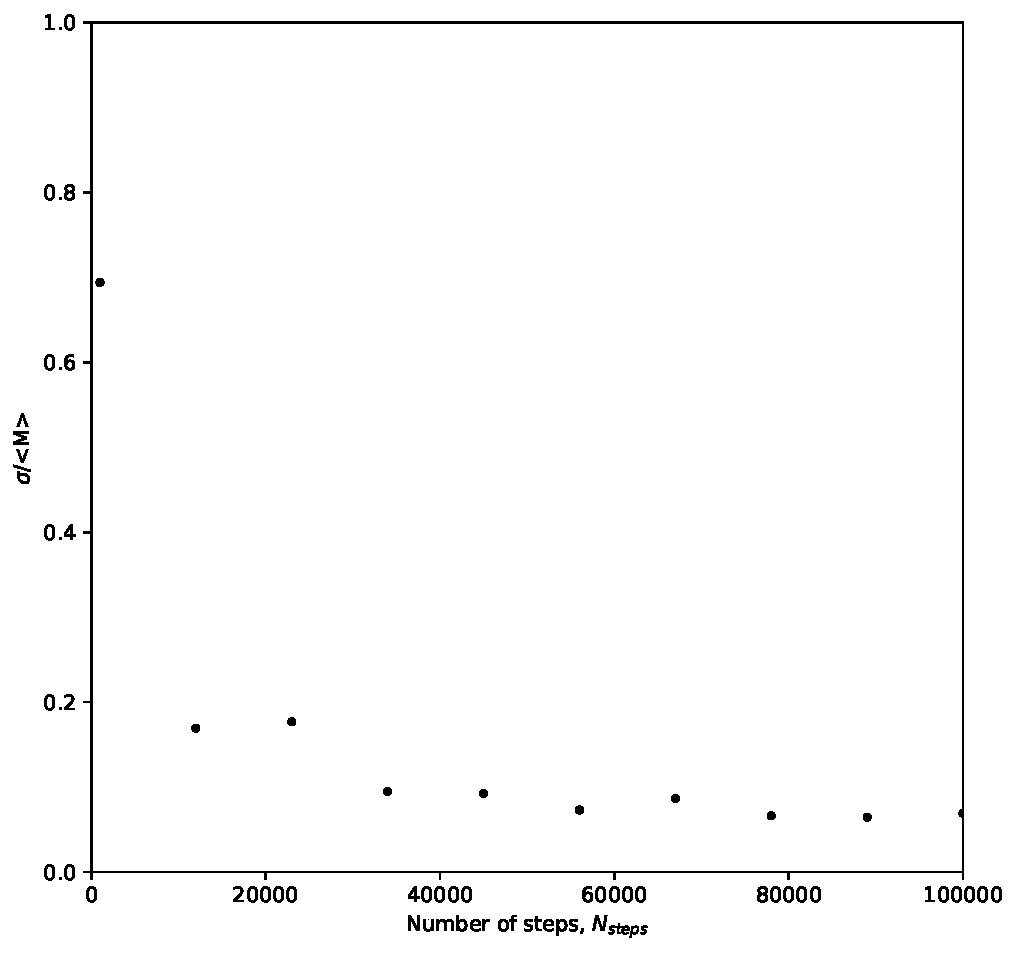
\includegraphics[width = 10 cm]{Comp_set_1/Confined_Lattice.pdf}
\caption{The ratio of standard deviatiob per average versus number of steps used.
}
\label{fig:confined_lattice}
\end{figure}  
As seen in the figure the process heads to zero suggesting our system is ergodic process since it should blow up spartically if the mean was always zero. 
\section{Problem 2: Monte-Carlo Pendulum}
Let's imagine a one dimensional lattice that loops back on itself. There is a force F(x) = -sin($\pi$(x-50)/50) that attracts the particles towards the center x = 50. Let's apply a 1D Ising model for this problem:
\subsection{a}
Deploying the model over three different betas:
\begin{figure}[H]
\centering
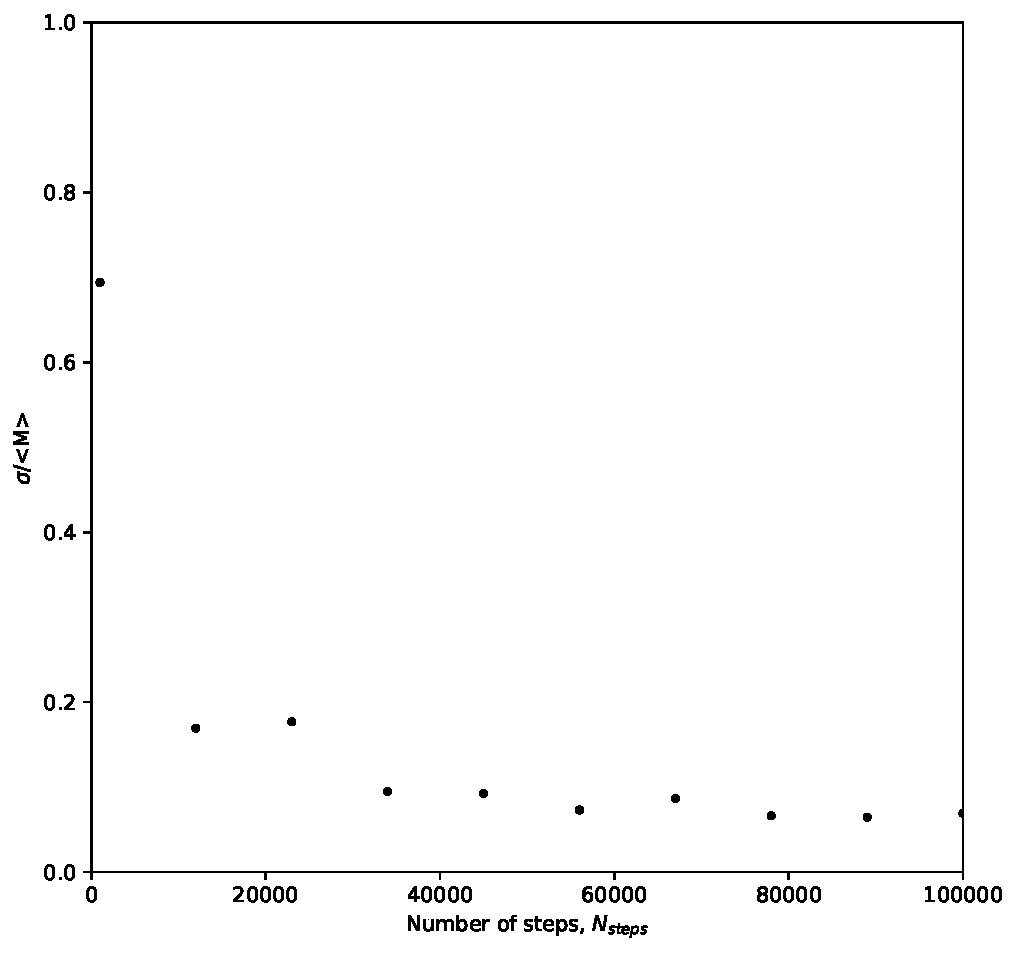
\includegraphics[width = 10 cm]{Comp_set_1/Confined_Lattice.pdf}
\caption{The ratio of standard deviatiob per average versus number of steps used.
}
\label{fig:confined_lattice}
\end{figure}  
\begin{figure}[H]
\centering
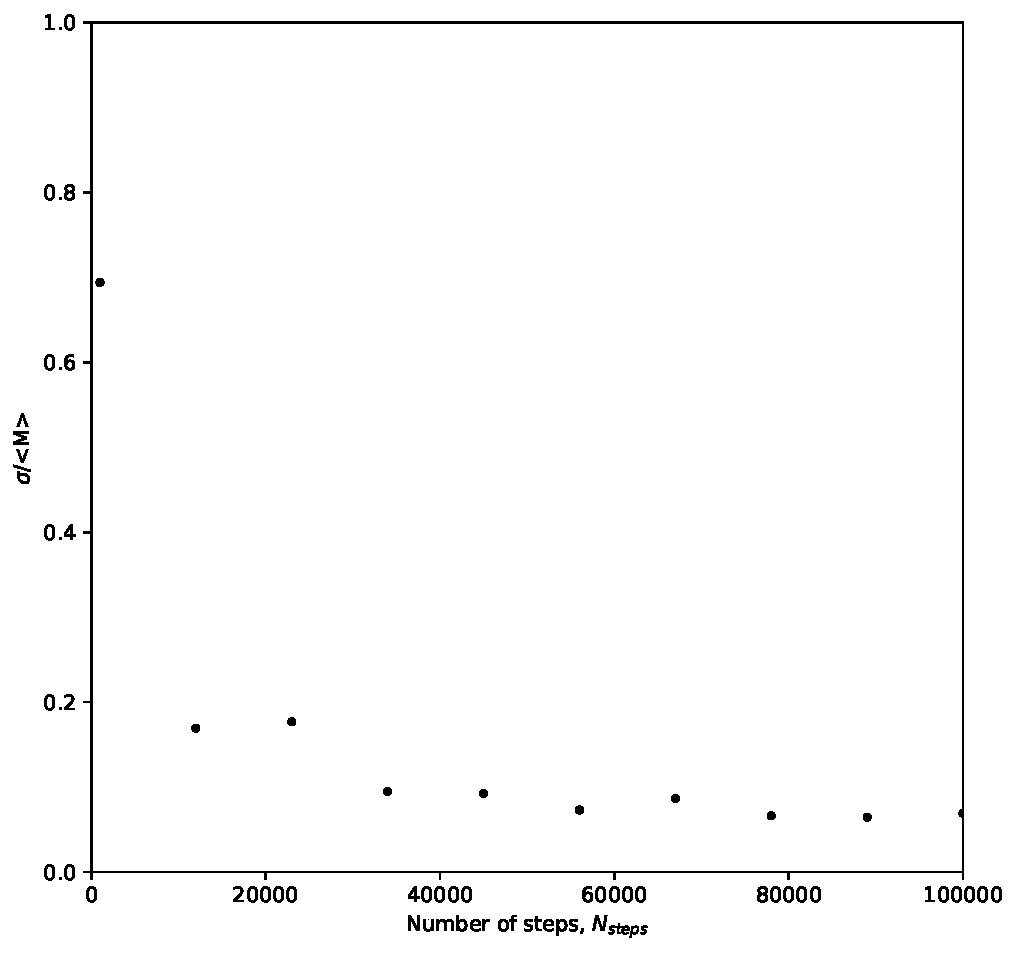
\includegraphics[width = 10 cm]{Comp_set_1/Confined_Lattice.pdf}
\caption{The ratio of standard deviatiob per average versus number of steps used.
}
\label{fig:confined_lattice}
\end{figure}  
As seen in the figure the
\begin{figure}[H]
\centering
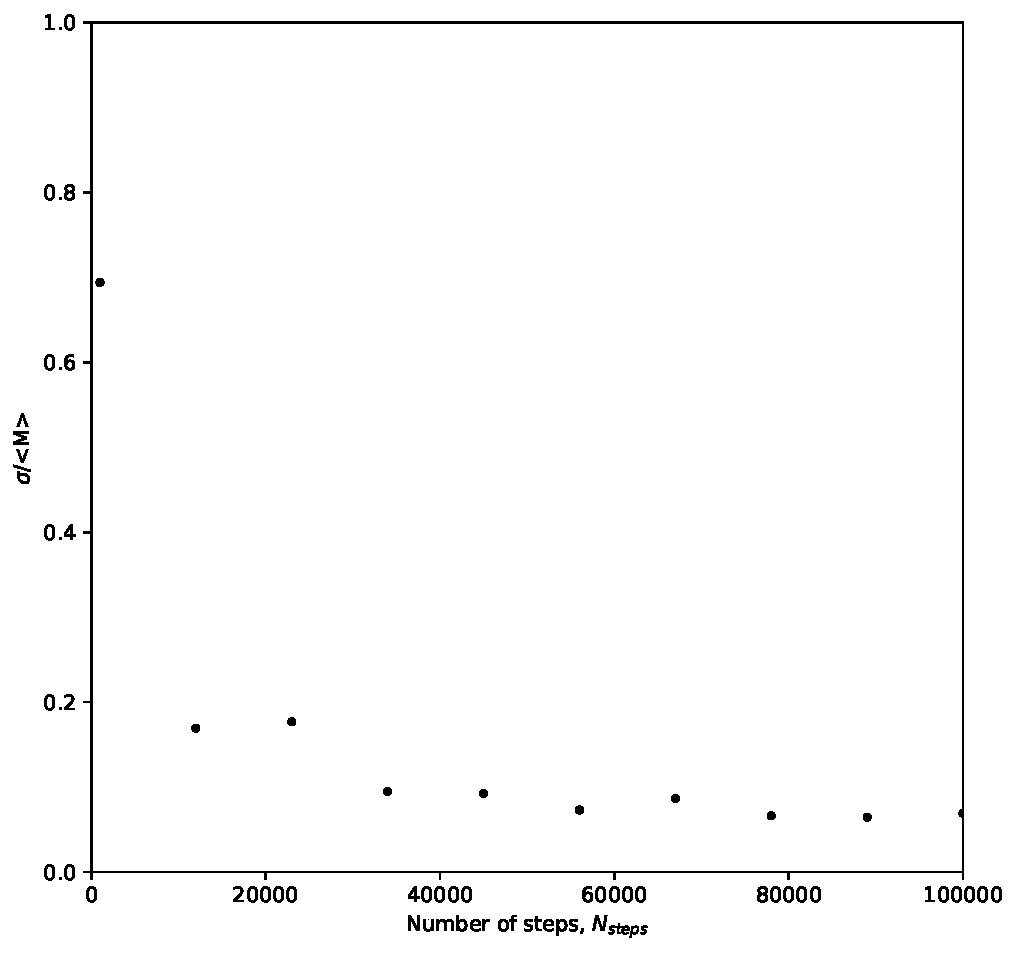
\includegraphics[width = 10 cm]{Comp_set_1/Confined_Lattice.pdf}
\caption{The ratio of standard deviatiob per average versus number of steps used.
}
\label{fig:confined_lattice}
\end{figure}  
As seen in the figure the
As seen in the figure the
\subsection{b}
\subsection{c}
\subsection{d}
\section{Problem 3}
\end{document}
